\documentclass[11pt, oneside]{article}   	% use "amsart" instead of "article" for AMSLaTeX format
\usepackage{geometry}                		% See geometry.pdf to learn the layout options. There are lots.
\geometry{letterpaper}                   		% ... or a4paper or a5paper or ... 
%\geometry{landscape}                		% Activate for rotated page geometry
\usepackage[parfill]{parskip}    		% Activate to begin paragraphs with an empty line rather than an indent
\usepackage{graphicx}				% Use pdf, png, jpg, or eps§ with pdflatex; use eps in DVI mode
								% TeX will automatically convert eps --> pdf in pdflatex		
\usepackage{amssymb}
\usepackage{amsmath}
\usepackage{float}


%SetFonts

%SetFonts


\title{Machine Learning 5800 Final Project}
\author{Luigi Patruno}
%\date{}							% Activate to display a given date or no date

\begin{document}
\maketitle

\abstract{In this paper I summarize the results and methodology of my analysis of the \textbf{Adult} data set. The goal of this project is to train and evaluate classification models in order to predict whether an individual earned above or below \$$50$k a year. My work includes an implementation of the Naive Bayes and regularized Logistic Regression models. Additionally, I used the regularized Logistic Regression and Support Vector Machine classifiers from the \textbf{scikit-learn} Python package. The most predictive model, an $L2$ regularized Logistic Regression that utilized $11$ of the $14$ features, achieved a test error of $.13589$ on a test set comprised of $10$\% of all data.}


\section{Introduction}

The \textbf{Adult}\footnote[1]{http://archive.ics.uci.edu/ml/datasets/Adult} data set consists of $32,561$ instances of data with $14$ features each. The data was extracted from the 1994 Census database and the feature set contains both numerical and categorical data. The prediction task associated with the set of data is to determine whether a person makes over \$$50$k a year in annual income. 

Although the data is relatively clean, I implemented several preprocessing steps before I trained classifiers. First, I converted the class labels from the string labels \texttt{<=50k}, \texttt{>50k} to integers $0$, $1$. This is relatively painless using the \textbf{pandas} package in Python. Further, since the machine learning algorithms from the \textbf{scikit-learn} module expect numerical input feature, I had to encode the categorical variables in the data set. For this task I employed a One-Hot encoding scheme. Essentially, this scheme converts a single categorical feature with $n$ distinct values into $n$ binary features. A categorical feature taking on particular value then corresponds to a tuple $(0,..,1,..,0)$ with a $1$ in the column corresponding to that particular feature value and $0$s elsewhere. Again, this was relatively painless using built-in functionality in \textbf{pandas} and \textbf{scikit-learn}.

Several features contained missing data.$1,836$ ($5.6$\%) samples were missing \textbf{workclass}, $1,843$ ($5.6$\%) samples were missing \textbf{occupation}, and $583$ ($1.8$\%) samples were missing \textbf{native-country}. In some schemes I treated the missing data as an additional value whereas in others I performed a feature reduction routine to reduce the dimensionality of the data. Of particular interest is a feature reduction implementation I used to reduce the number of relevant features from $14$ to $11$ using an $L2$ regularized Logistic Regression model. This procedure led to my most predictive model.

I trained an evaluated various classifiers. I implemented both a multi-dimensional Naive Bayes classifier and a regularized Logistic Regression classifier. Due to an inefficient implementation of the Logistic Regression classifier, however, I opted to go with the built-in regularized Logistic Regression algorithm in \textbf{scikit-learn}. I also trained and evaluated various SVM classifiers, again from \textbf{scikit-learn}. 

Below is a summary of the most predictive models for each class of algorithm:

\begin{center}
\begin{tabular}{ l || l  }
    \hline
    \textbf{Algorithm} & \textbf{Test error} \\ \hline
    Naive Bayes & $.152$   \\ \hline
    Logistic Regression $L1$ &  $.1406$     \\ \hline
    Logistic Regression $L2$ &  $.136$    \\ \hline
    Support Vector Machine &  $.201$     \\ \hline
\end{tabular}
\end{center}


\section{Methods}

In order to build an effective predictive model for the \textbf{Adult} data set, I built and evaluated several different types of classifiers. The classification models I chose are the Naive Bayes, Logistic Regression and Support Vector Machine classifiers. I evaluated each classifier's performance by learning model parameters on a training set and computing the classification error on a held-out test set. For each of the Naive Bayes and Logistic Regression classifiers built, I also implemented various feature selection/reduction routines. I retrained classifiers using these feature selection routines and evaluated these models by calculating a test error. What follows below is a description of each classifier, the model parameter and hyper-parameter tuning procedure, and the feature selection/reduction procedures.

\subsection{Naive Bayes}

Naive Bayes is a conditional probability model that relies on the application of \textbf{Bayes Theorem} and the assumption that each feature $ \mathbf{X_i} $ is conditionally independent of every other feature conditioned on the class. Therefore, we calculate the probability of a class $ Y $ given features $ X_1, X_2, ..., X_n $ as 

\[ p(Y| X_1, X_2, ..., X_n) = p(Y|X_1) p(Y|X_2)...p(Y|X_n). \]

Although the assumption of conditional independence among the features are often violated, the Naive Bayes model often works well in practice. Further, due to the conditional independence assumption, the number of parameters to learn grows linearly with the number of features. 

I decided to implement my own version of the Naive Bayes classifier. This implementation can be found in \texttt{naivebayes.py}. The method \texttt{learn\_parameters} is responsible for learning the model parameters. The method works by looping through each of the features involved and calculating model parameters for numerical and categorical data. If a feature is a numerical feature, the method learns the feature's mean and standard deviation, conditioned on the class. For instance, the method learns the mean and standard deviation of the \textbf{age} feature for the data samples that fall within class $ 0 $ and class $ 1 $. For categorical data, I simply calculate the fraction of training samples that take on a particular feature value, per class. For example, for each value in feature \textbf{native-country}, the Naive Bayes model learns the fraction of all samples that take on that particular value, for each of the samples in both classes.

Since several features contain missing data points, I provide an option to learn model parameters ignoring these features. That is, in order to learn Naive Bayes model parameters for all features that do not contain missing values, instantiate the Python object as follows:

\begin{verbatim}
nb = NaiveBayes(ignore_missing=True)
\end{verbatim}
.The default behavior is to learn model parameters for all features. The corresponding Python object is instantiated as follows:

\begin{verbatim}
nb = NaiveBayes()
\end{verbatim}
. Aside from the number of feature used to train the model, I also experimented with the size of the training set and testing set. Specifically, I trained and evaluated models with a training set size comprised of $50$\%, $60$\%, $...$, $90$\% of the total data. For each training set size, I built two separate classifiers: one that used all of the features, and one excluding features that contained missing values. A driver performing the Naive Bayes analysis can be found in \texttt{run\_naivebayes.py}. The results of this analysis can be found in file \texttt{results\_naivebayes.txt}.

\subsection{Logistic Regression}

Logistic Regression is a classification algorithm that measures the relationship between the categorical dependent variable and one or more independent variables by estimating probabilities using a logistic function 
\footnote[2]{https://en.wikipedia.org/wiki/Logistic\_regression}. 
That is, we can learn parameters for Logistic Regression through Maximum Likelihood Estimation by maximizing the likelihood defined by

\[ L(y|\mathbf{x}; \mathbf{w}) = \prod_i{1-g(\mathbf{x}^i;\mathbf{w})^{(1-y^i)}g(\mathbf{x}^i;\mathbf{w})^{y^i}} \]
where
\[ g(\mathbf{x}^i,\mathbf{w}) = \frac{1}{1+e^{-\mathbf{x}^T\mathbf{w}}} \]
and our  our class probabilities are

\begin{align}
    p(y=0|\mathbf{x};\mathbf{w}) &= 1-g(\mathbf{x}^T\mathbf{w}) \\ 
    p(y=1|\mathbf{x};\mathbf{w}) &= g(\mathbf{x}^T\mathbf{w})
\end{align}
.The update rule for the Maximum Likelihood Estimation is given by 
\[ \mathbf{w}_j \leftarrow \mathbf{w}_j + \epsilon \mathbf{x}_j^i(y^i - g(\mathbf{x}^T\mathbf{w})) \]
where we loop over each data point $(y^i, \mathbf{x}^i)$ and update each weight $\mathbf{w}_j$.

We can choose to regularize our model to reduce overfitting and punish outliers within the data. 
For example, $L1$ regularization seeks to minimize all learned weights. The update rule for $L1$ regularization is
\[ \mathbf{w}_j \leftarrow \mathbf{w}_j + \epsilon \bigg[\mathbf{x}_j^i(y^i - g(\mathbf{w}^T\mathbf{x}^i)) 
- \frac{\text{sign}(\mathbf{w}_j)}{\lambda N} \bigg] \]
$L2$ regularization, on the other hand, seeks to minimize the number of non-zero weights. It's update rule is given by
\[ \mathbf{w}_j \leftarrow \mathbf{w}_j + \epsilon \bigg[\mathbf{x}_j^i(y^i - g(\mathbf{w}^T\mathbf{x}^i)) 
- \frac{\mathbf{w}_j}{\lambda N} \bigg]. \]

I first decided to implement the Logistic Regression classifier with the option of fitting a model with no regularization, or the option of using $L1$ or $L2$ regularization. This implementation is contained within \texttt{logisticregression.py} and a sample driver is found within \texttt{run\_logistic\_regression\_implementation.py}. Although I implemented the routine, I was unhappy with the performance of my implementation when compared to the implementation found in the \textbf{scikit-learn} open-source Python package. Therefore, I decided to use the \textbf{scikit-learn} for my analysis. I've included my implementation for the sake of completeness. Note, however, that my results are from the \textbf{scikit-learn} package.

First, I trained and evaluated several Logistic Regression classifiers using $L1$ regularization. I split the data into training and test sets ($80$\%, $20$\% splits) and learned model parameters and hyper-parameters by training the models on the training sets and evaluating them by calculating classification error on the test sets. I varied the regularization hyper-parameter $ \lambda $ over the grid of points from $.1$ to $10$ in increments of $.1$, from $10$ to $100$ in increments of $10$, and from $100$ to $1000$ in increments of $100$ for a total of $114$ different models. Since $L1$ regularization seeks to minimize all learned weights $\mathbf{w}_j$, feature subset selection is performed implicitly when training the model. Hence, I performed no further feature selection. A driver performing the $L1$ analysis can be found in \texttt{run\_logistic\_l1.py}. The results of this analysis can be found in file \texttt{results\_logistic\_l1.txt}.

I also trained and evaluated several Logistic Regression classifiers using $L2$ regularization. This time however, I implemented a feature reduction scheme. This implementation can be found in \texttt{featureselection.py}. I will explain the basic mechanics of this routine as it is quite involved. In order to perform feature reduction while simultaneously tuning model the $L2$ hyper-parameters $ \lambda $, I split the data set into three parts; a training set ($80$\%) for learning model parameters, a validation set ($10$\%) for fine tuning model hyper-parameters, and a test set ($10$\%) for evaluating the model. The details of this approach can be found in 
\footnote[3]{G. James, D. Witten, T. Hastie, R. Tribshirani. \textit{An Introduction to Statistical Learning}. pg. $248$}.
I outline the algorithm below:
\begin{verbatim}
For each n from 14..1:
    size_n_subsets = The set of all subsets of features of size n
  
    For each subset in size_n_subsets:
        Train a classifier on the training set
        Evaluate the classifier on the validation set
    
    min_n_error = the minimum test error over size_n_subsets
  
min_n = minimum over all min_n_error
best_n_subset = The set of all subsets of features of size min_n

For subset in best_n_subset:
    Train a classifier on the training and validation set
    Evaluate the error on the test set
    
Retrieve the features and error that minimized the error in the previous loop
\end{verbatim} 
As stated in \textit{An Introduction to Statistical Learning}, in order for a feature reduction scheme to yield accurate estimates of the test error, we must "use only the \textit{training observations} to perform all aspects of model-fitting including variable selection. Therefore, the determination of which model of a given size is best must be made using \textit{only the training observations}."  This procedure ensures that we arrive at the best possible estimates for test error. I varied the regularization hyper-parameter $ \lambda $ over the grid of points from $.1$ to $5$ in increments of $.1$, and also looked at $ \lambda \in \{ 10, 50, 100, 200 \} $. I also varied the number of iterations to train the logistic regression $ \text{max\_iter} \in \{ 10,50,100,200 \}$. Hence, a total of $54 \times 3 = 162$ models were fit and evaluated. A driver performing the $L2$ analysis can be found in \texttt{run\_logistic\_l2\_feature\_selection.py}. The results of the feature reduction routine can be found in file \texttt{results\_logistic\_l2.txt}.

\subsection{Support Vector Machine}

The Support Vector Machine classifier constructs a set of hyperplanes in the feature space that can be used for classification. SVM differs from the Logistic Regression in that the hyperplane found is the hyperplane that maximizes the distance to the nearest training point in any class. Further, nonlinear boundaries can be found by using the kernel trick. For the sake of brevity, I am excluding a more in depth review of the mechanics of the Support Vector Machine optimization process. A sc

For my analysis, I trained and evaluated several SVM classifiers. I split the data into training and test sets ($80$\%, $20$\% splits) and learned model parameters and hyper-parameters by training the models on the training sets and evaluating them by calculating classification error on the test sets.  I varied the penalty on the error term $ \epsilon $ by looking at values  $ \epsilon \in \{ .1,1 \}  $. I also trained several other classifiers using the Gaussian radial basis kernel. For these models I varied $ \epsilon $ from $.1$ to $1$ in increments of $.1$ and also included $\epsilon \in \{ 10, 100 \}$. Hence, I trained a total of $14$ SVM classifiers. A driver performing the SVM analysis can be found in \texttt{run\_svm.py}. The results of the feature reduction routine can be found in file \texttt{results\_svm.txt}.
 
\section{Results}
 
The results of the Naive Bayes analysis are in Figure $1$. As the training set size grew, the test error decreased. This is expected as learning from more data decreases the variability of the possible feature values. The most performant model was achieved with a training set comprised of $90$\%. This model also used all of the feature values, including features containing missing data. The test error on this set was $.152$. 


\begin{figure}[!ht]
\caption{Naive Bayes Results}

\begin{center}
\begin{tabular}{ l | l || l }
    \hline
    Train Set Size & Ignore features with missing values & Test Error \\ \hline
    $50$\% & True & $.169$   \\ \hline
    $50$\% & False &  $.162$     \\ \hline
    $60$\% & True &  $.170$    \\ \hline
    $60$\% & False &  $.162$     \\ \hline
    $70$\% & True &  $.169$     \\ \hline
    $70$\% & False &  $.160$     \\ \hline
    $80$\% & True &  $.166$     \\ \hline
    $80$\% & False &  $.156$     \\ \hline
    $90$\% & True &  $.165$     \\ \hline
    $90$\% & False &  $.152$     \\ \hline
\end{tabular}
\end{center}
\end{figure}

The results of the Logistic Regression with $L1$ regularization analysis are summarized in Figure $2$.  Although there seems to be a lot of variability in the Test Error as we vary over the regularization strength $ \lambda $, the test error only varies within the range $ [.1406, .1437]$ with the most predictive model having $ \lambda = 1.1$.

\begin{figure}[H]
\caption{Logistic Regression L1 regularization}
\begin{center}
  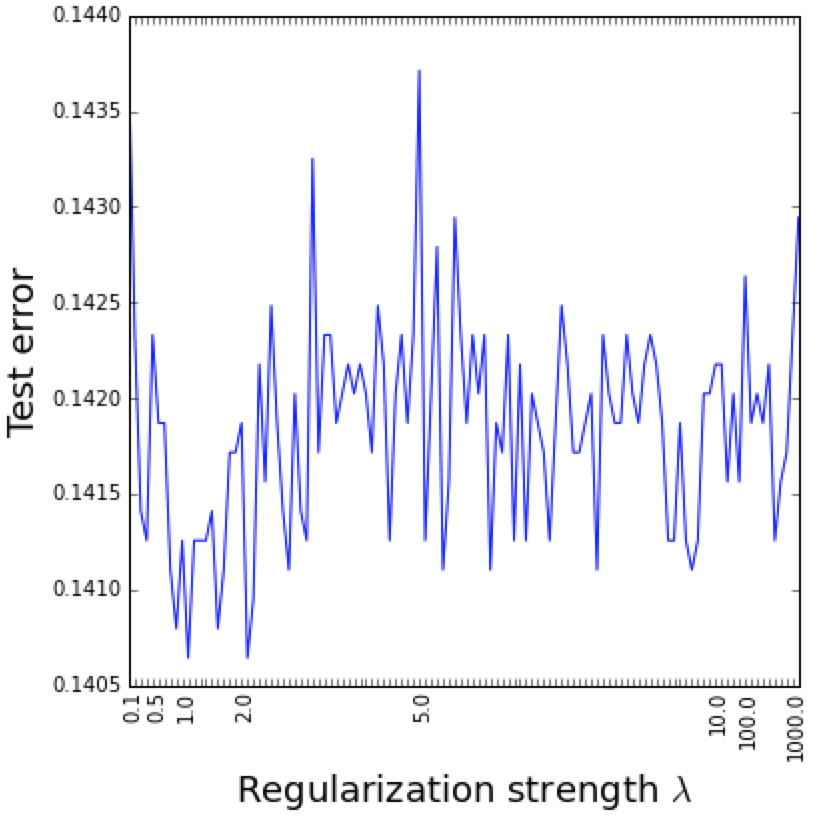
\includegraphics[scale=.5]{logistic_regression_l1}
\end{center}
\end{figure}

The most predictive models in my analysis were the $L2$ regularized Logistic Regression models that were trained with the feature reduction scheme. First, although the test error decreased when increasing the number of training iterations from $10$ to $50$, there was no improvement whatsoever when increasing the number of iterations to $100$ or $200$ (see Figure $3$). If we examine one of these models more closely, as in Figure $4$, we see that the minimum test error occurs when $ \lambda =  4.1$. This was my most predictive model with a test error of $.13589$.  The features selected by the feature reduction scheme are [\textbf{age}, \textbf{workclass}, \textbf{education-num}, \textbf{occupation}, \textbf{relationship}, \textbf{race}, \textbf{sex}, \textbf{capital-gain}, \textbf{capital-loss}, \textbf{hours-per-week}, \textbf{native-country}].

\begin{figure}[H]
\caption{Logistic Regression L2 regularization varying number of iterations}
\begin{center}
  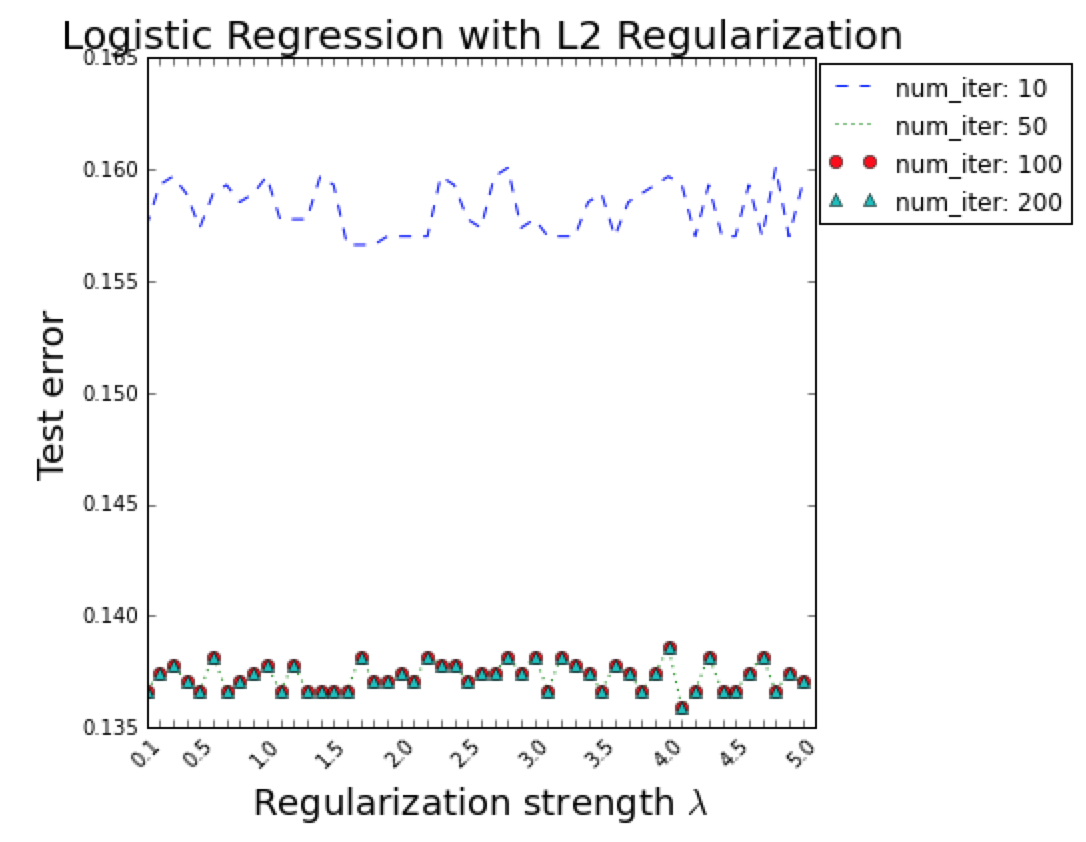
\includegraphics[scale=.6]{logistic_regression_l2_num_iter}
\end{center}
\end{figure}

\begin{figure}[H]
\caption{Logistic Regression L2 regularization}
\begin{center}
  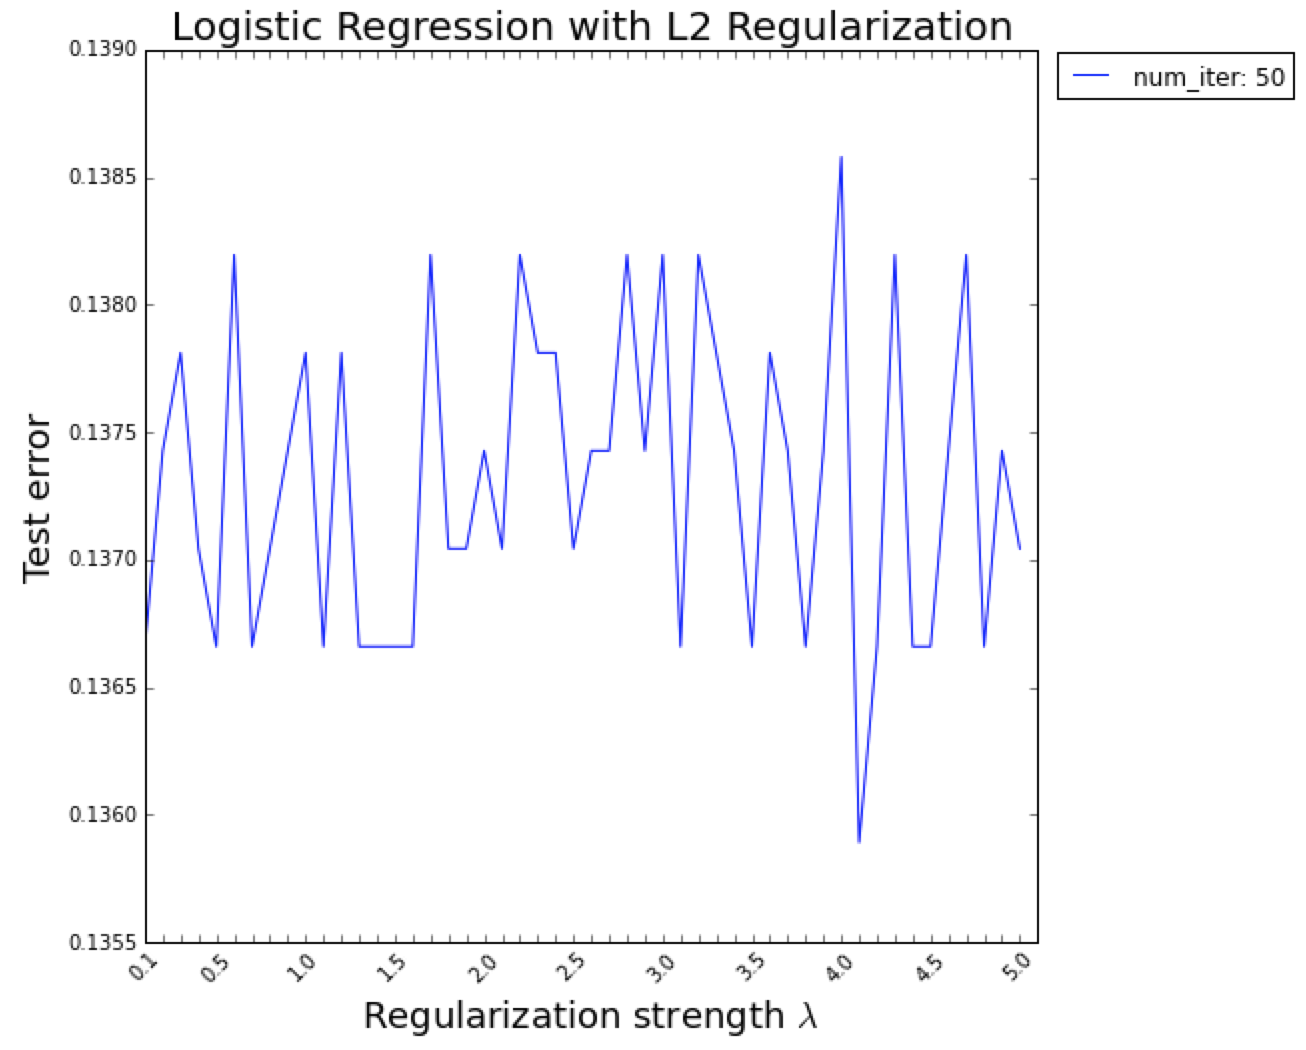
\includegraphics[scale=.4]{logistic_regression_l2}
\end{center}
\end{figure}


The SVM classifiers were the least predictive models (Figure $5$). The most predictive SVM model used a linear kernel and applied a penalty of $.1$ to misclassified points. The test error of this model was $.20098$.

\begin{figure}[H]
\caption{SVM Results}

\begin{center}
\begin{tabular}{ l | l || l }
    \hline
    Kernel & Error Penalty & Test Error \\ \hline
    Linear & $.1$ & $.201$   \\ \hline
    Linear & $1$ &  $.201$     \\ \hline
    Radial Basis & $.1$ &  $.241$    \\ \hline
    Radial Basis & $.2$ &  $.241$     \\ \hline
    Radial Basis & $.3$ &  $.241$     \\ \hline
    Radial Basis & $.4$ &  $.241$     \\ \hline
    Radial Basis & $.5$ &  $.242$     \\ \hline
    Radial Basis & $.6$ &  $.240$     \\ \hline
    Radial Basis & $.7$ &  $.239$     \\ \hline
    Radial Basis & $.8$ &  $.241$     \\ \hline
    Radial Basis & $.9$ &  $.244$     \\ \hline
    Radial Basis & $1$ &  $.247$     \\ \hline
    Radial Basis & $10$ &  $.257$     \\ \hline
    Radial Basis & $100$ &  $.258$     \\ \hline
    Radial Basis & $1000$ &  $.258$     \\ \hline
    
\end{tabular}
\end{center}
\end{figure}

\section{Conclusion}

Overall, this final project was a fantastic way to apply the methods I've learned over a semester of CISC 5800. I was able to code up a repeatable set of experiments for evaluating the efficacy of many predictive models and I learned a lot about the theory and applicability of different algorithms. One of the more interesting things I took away from this project is that simple models are sometimes more predictive than more complicated routines. For instance, my implementation of the Naive Bayes model far outperformed both the linear and nonlinear SVM models. Even more importantly, the Naive Bayes model learned its parameters way faster than the SVM models. Aside from this, I recognize the importance of coming up with good features in order to improve model predictiveness. I'd like to thank Dr. Leeds for a great semester. I truly enjoyed his class.



\end{document}  

























